\subsection{Cơ sở lý thuyết về Thị giác Máy tính (CV)}
\begin{frame}
\frametitle{Định nghĩa và Mục tiêu}
\begin{block}{Định nghĩa}
\textbf{Thị giác Máy tính (CV)}: Lĩnh vực AI cho phép máy tính xử lý, phân tích và diễn giải hình ảnh/video, mô phỏng thị giác con người.
\end{block}

\begin{block}{Mục tiêu}
\begin{itemize}
\item Tái tạo khả năng nhận thức thị giác với tốc độ, độ chính xác và quy mô vượt trội.
\item Ứng dụng trong \TENLUANVAN, đặc biệt là \textbf{Ước lượng Tư thế Người (HPE)}.
\end{itemize}
\end{block}
\end{frame}

\begin{frame}
\frametitle{Pipeline Cơ bản của Hệ thống CV}
\begin{block}{Quy trình}
\begin{enumerate}
\item \textbf{Thu nhận dữ liệu}: Thu thập ảnh/video từ camera.
\item \textbf{Tiền xử lý}: Chuẩn hóa kích thước, điều chỉnh sáng/tương phản, giảm nhiễu.
\item \textbf{Trích xuất đặc trưng}: Chuyển pixel thành đặc trưng trừu tượng (cạnh, góc, kết cấu).
\item \textbf{Phân tích và quyết định}: Phân loại, nhận dạng hoặc ước lượng tư thế.
\end{enumerate}
\end{block}

\begin{exampleblock}{Minh họa}
\begin{center}
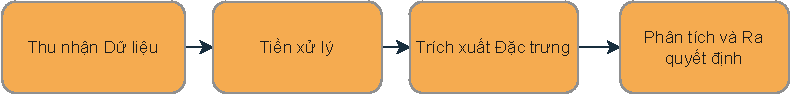
\includegraphics[width=0.9\textwidth]{images/vision_flow-crop.pdf}
\caption{Quy trình tổng thể của hệ thống CV.}
\label{fig:cv_pipeline}
\end{center}
\end{exampleblock}
\end{frame}

\begin{frame}
\frametitle{Phân loại Bài toán CV}
\begin{block}{Các bài toán cốt lõi}
\begin{itemize}
\item \textbf{Phân loại Ảnh}: Gán nhãn cho toàn bộ ảnh (VD: "Người", "Xe").
\item \textbf{Phát hiện Đối tượng}: Xác định vị trí và nhãn bằng hộp giới hạn.
\item \textbf{Phân đoạn Ảnh}:
\begin{itemize}
\item \textbf{Ngữ nghĩa}: Gán nhãn từng pixel (VD: Đường, Cây).
\item \textbf{Thể hiện}: Phân biệt các cá thể cùng lớp.
\end{itemize}
\item \textbf{Ước lượng Tư thế Người (HPE)}: Xác định tọa độ \textbf{khớp keypoint} để phân tích chuyển động.
\end{itemize}
\end{block}
\end{frame}

\begin{frame}
\frametitle{Mô hình Học sâu: CNN}
\begin{columns}
\begin{column}{0.5\textwidth}
\begin{itemize}
\item \textbf{Mạng Nơ-ron Tích chập (CNN)}: Kiến trúc chủ đạo cho xử lý ảnh.
\item \textbf{Phép tích chập}: Trích xuất đặc trưng cục bộ:
\begin{equation}
\footnotesize
(I * K)(i, j) = \sum_{m} \sum_{n} I(i-m, j-n) K(m, n)
\end{equation}
\item \textbf{Phép gộp}: Giảm kích thước, tăng tính bền vững (VD: Max Pooling).
\end{itemize}
\end{column}

\begin{column}{0.45\textwidth}
\begin{figure}
\centering
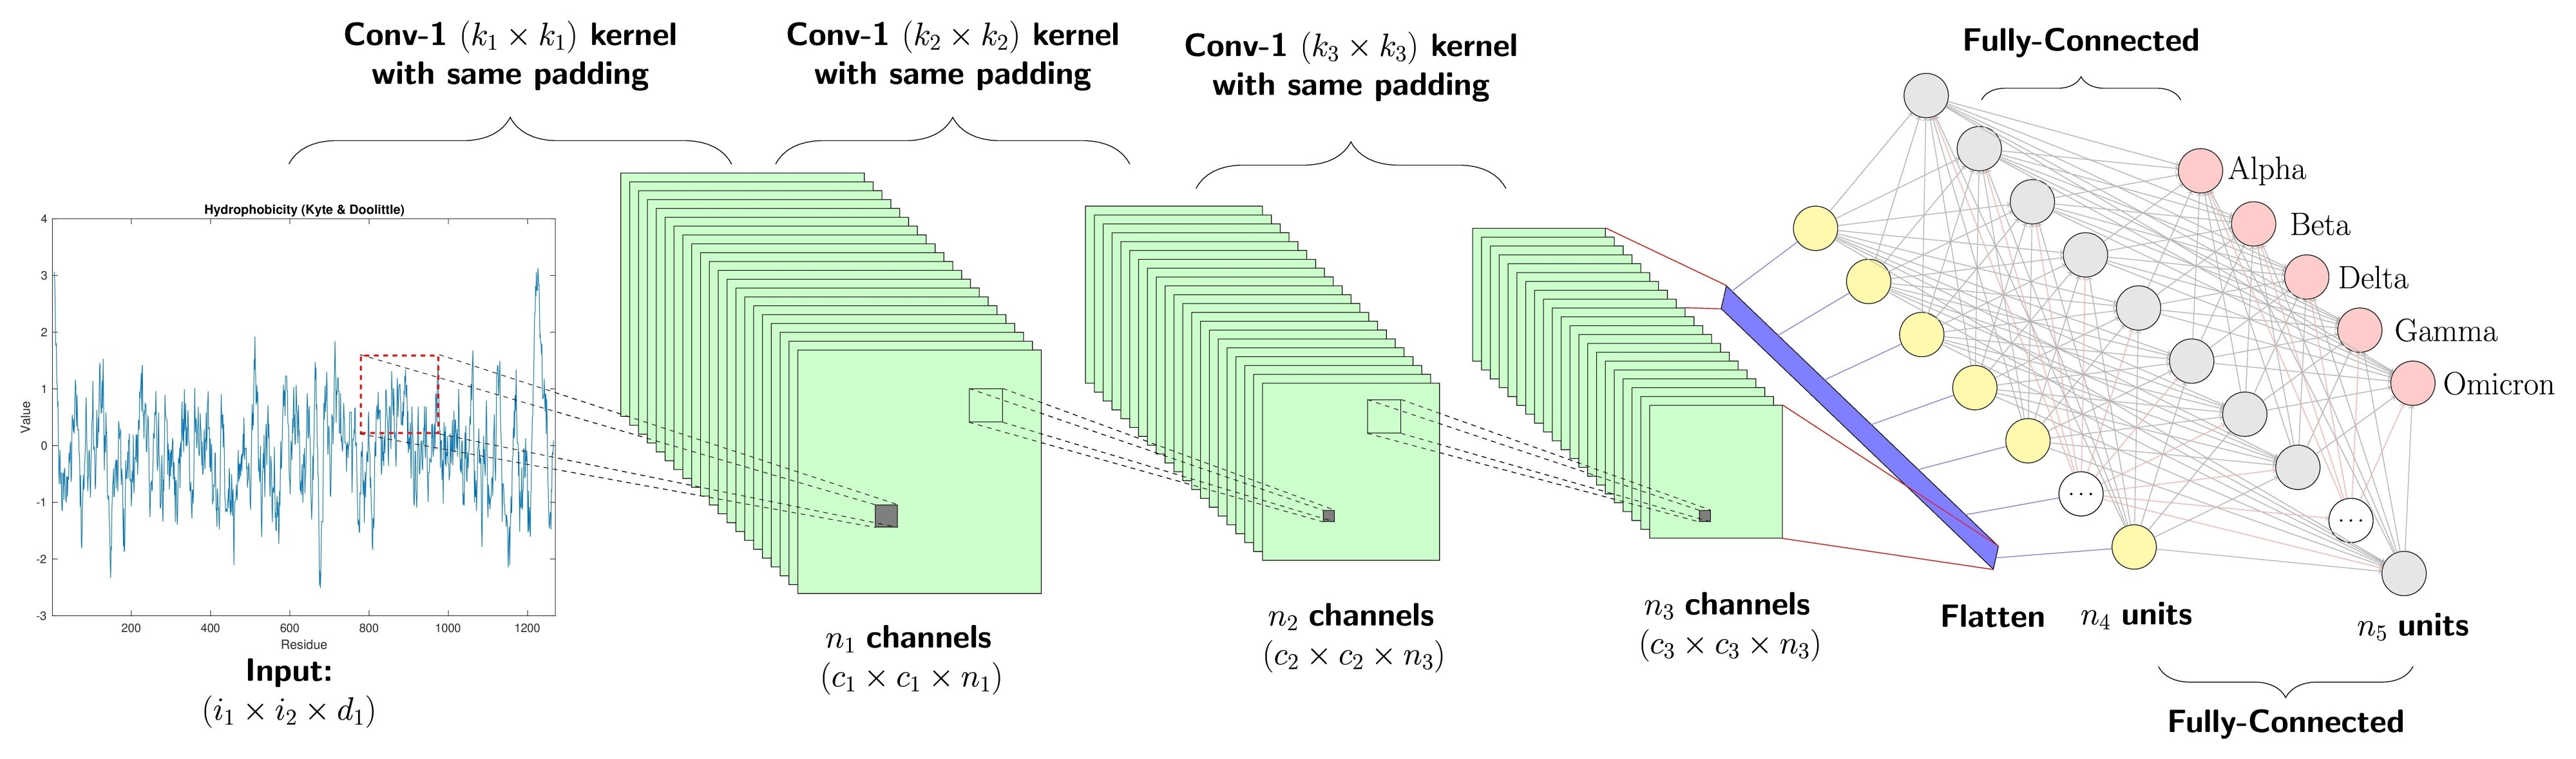
\includegraphics[width=\textwidth]{images/2_2_convolution.jpeg}
\caption{Phép tích chập và gộp.}
\label{fig:cnn_ops}
\end{figure}
\end{column}
\end{columns}
\end{frame}

\begin{frame}
\frametitle{Mô hình Học sâu: Vision Transformer}
\begin{columns}
\begin{column}{0.5\textwidth}
\begin{itemize}
\item \textbf{Vision Transformer (ViT)}: Chia ảnh thành \textbf{miếng vá}, xử lý như token.
\item \textbf{Tự chú ý (Self-Attention)}:
\begin{equation}
\footnotesize
\text{Attention}(Q, K, V) = \text{softmax}\left(\frac{QK^T}{\sqrt{d_k}}\right)V
\end{equation}
\item Học quan hệ toàn cục, vượt giới hạn của CNN.
\end{itemize}
\end{column}

\begin{column}{0.45\textwidth}
\begin{figure}
\centering
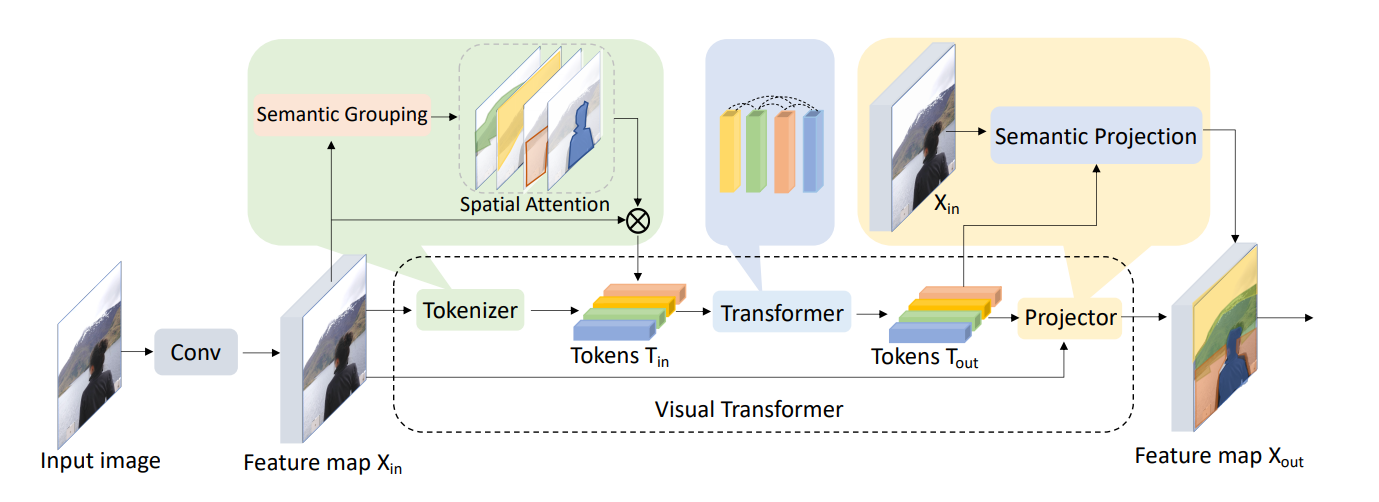
\includegraphics[width=\textwidth]{images/visual_transformer.png}
\caption{Kiến trúc ViT.}
\label{fig:vit_arch}
\end{figure}
\end{column}
\end{columns}
\end{frame}

\begin{frame}
\frametitle{Tập dữ liệu và Metrics Đánh giá}
\begin{block}{Tập dữ liệu}
\begin{itemize}
\item \textbf{ImageNet}: Phân loại ảnh (>14 triệu ảnh).
\item \textbf{COCO}: Phát hiện, phân đoạn đối tượng.
\item \textbf{MPII, COCO Keypoints}: Ước lượng tư thế người (HPE).
\end{itemize}
\end{block}

\begin{block}{Metrics đánh giá}
\begin{itemize}
\item \textbf{IoU}: Đo độ trùng khớp hộp giới hạn.
\item \textbf{mAP}: Trung bình độ chính xác cho phát hiện đối tượng.
\item \textbf{F1-score}: Cân bằng Precision và Recall.
\item \textbf{OKS}: Đo độ chính xác khớp trong HPE.
\end{itemize}
\end{block}
\end{frame}
